\section{P2P Identification Schemes}
\subsection{Plain PKI scheme}
\subsection{Peerson Username/Password scheme}
%
%% introduction of identification schemes. Par 2: proposed username/password identification schemes. Part 3: securing the network protocols. Part 4: Pending issues.
\paragraph{Account registration}
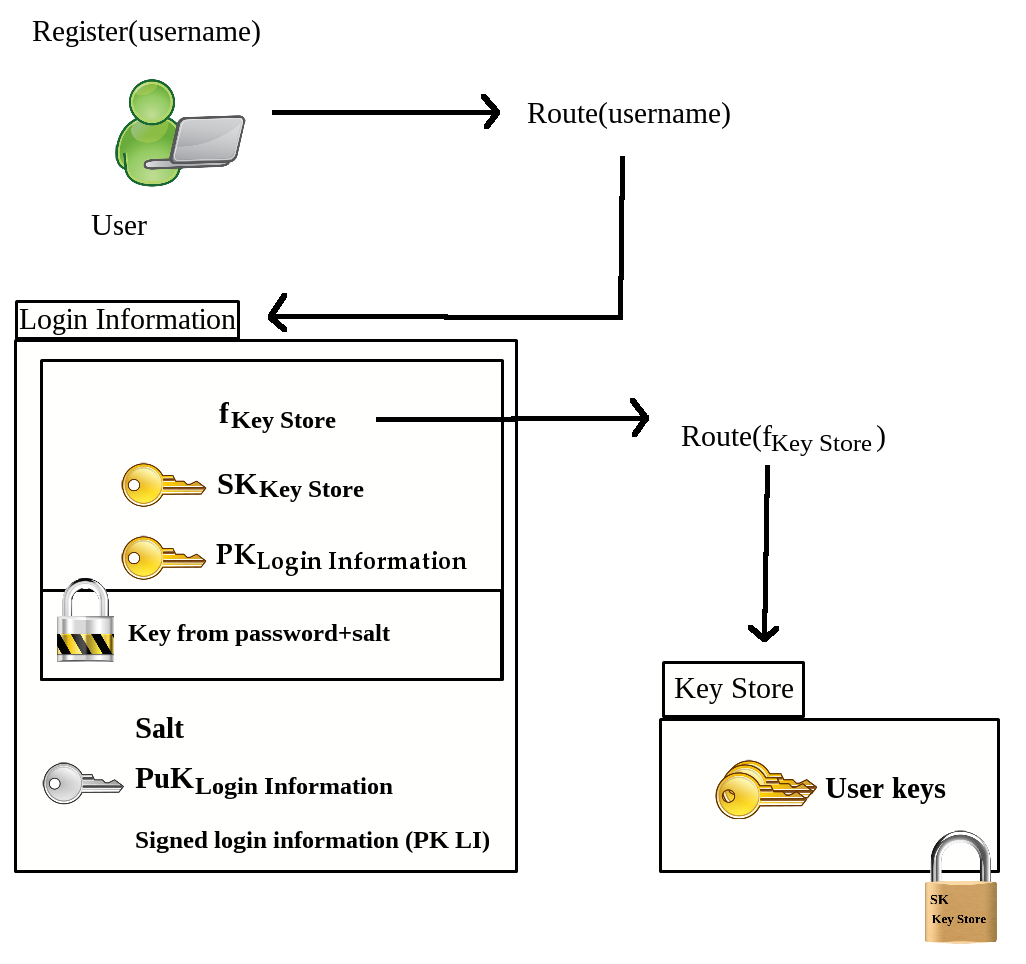
\includegraphics[width=14cm]{../img/user_registration}\\
To register a new user account, the user first
has to choose a \textit{username} and a \textit{password}.

% key store file
Considering a key-based authentication, the user creates a \textit{key store file}, containing all the
keys used by the P2P application the user wants to log in to.
The user generates a cryptographic key to authenticate the write operations
that will be made in the file, and store this key along with the others in the
\textit{key store file}.


% encryption and store of the key store file
The user then creates a \textit{symmetric key KKS} ,
encrypts the file content with this key and puts the ciphertext
into the storage, obtaining a \textit{file name fKS} . Now, the user
creates a \textit{login information file} by creating a random
byte string \textit{salt}, deriving a \textit{symmetric key KLI} from the user
\textit{password} and the \textit{salt}.
Using the new \textit{ symmetric key KLI}, the user encrypts the \textit{file name fKS},
the \textit{symmetric key KKS} and the \textit{cryptographic key to
authenticate the write operations KW}.
 The salt and the three encrypted values are put
into the storage, obtaining a file name fLI . The salt is stored
in plaintext, so that the user later can derive the decryption
key KLI by only providing the password. Finally, the user
performs the write-once operation put on the DHT with
uname as key and fLI as value.

%unique username
If the username was taken,
the user is prompted for a new username.

%finish
Once all operations
have succeeded, the user is registered in the system.


\paragraph{Sign-in}
The user uses his username to find and retrieve his \textit{login information
file}. Then, using his \textit{password} and the \textit{salt} included in the
\textit{login information file}, obtains the \textit{file name fKS} used to
route back to where the \textit{key store file} is stored.  Lastly, uses the
\textit{symmectric key KKS} to dencrypt the \textit{key store file} and recover
his user keys.

\paragraph{Logout}
The system does not have something like a "session" to maintain; the only way
to identify an user is by his keys that are obtained by the identification
process.

%%%%%%%%%%%%%%% REWRITE THISSSSSSSSSSSSSSSSSSSSSSSSSSSSSSSS
 To log out from the system, the user does not have to interact
with the DHT or the storage system. Simply wiping her local
cache from application data and all key material restores the
pre-login state. If the user chose to remember the login on a
device, the corresponding device login information file FDL
can also be deleted from the storage.
 A problem related to logging out is revoking remembered
credentials on another device, e. g., a user’s stolen phone. To
accomplish this, we first run the password change operation,
which locks out all devices with remembered logins, because
he key store key KKS changed (as well as the filename fKS ).
Next, we use the device mapping devmap to inform all devices
about the new key (and filename), except the device that is to
be revoked. To inform a device about the change, we update
the corresponding values in the device’s login information file
 FDL which can be accessed from the device by using the
locally stored credentials.
 Algorithm 4 describes this necessary extension. After run- the password change
operation, all devices that not ning shouldbe revoked and that have remembered
logins (and therefore are devmap) referenced in the device mapping are
processed. The device login information filename fDL and its key KDL are read,
and the new key store key KKS new and filename fKS new are written to the
device login information file FDL, encrypted under the device key KDL.
Finally, the modified devmap is saved back to the login information file FLI.
%%%%%%%%%%%%%%% REWRITE THISSSSSSSSSSSSSSSSSSSSSSSSSSSSSSSS
 



\paragraph{Password Change}
To change the password, the user has to rewrite his \textit{login information
file}.


%%%%%%%%%%%%%%% REWRITE THISSSSSSSSSSSSSSSSSSSSSSSSSSSSSSSS
Before the user can change the password, she must log in using her password to
obtain KLI . With this information, the password change can be accomplished
(see Algorithm 3): the user is asked for a new password and a new salt is
generated. The key-derivation function is used to generate a new key KLI new
for the login information file. Then, the content of the key-store file is
fetched and decrypted (with the old key). A new key KKS new is generated and
used for encrypting the key-store content again before it is saved to the
storage system, obtaining a new filename fKS new.
Finally, the login information file
is updated: fKS new, KKS new, the write credential KW as well as a new empty
device mapping devmapnew are encrypted with the new key KLI new.
  Together with the new salt, this ciphertext is written to the distributed
storage, using the reference fLI and the credential KW, to authenticate the
write operation. Lastly, the keys stored in the key store should be updated by
the application using our P2P protocol.  See Section VI-E for a discussion. At
this point, old device login information files can also be deleted from the
storage to reclaim space.
%%%%%%%%%%%%%%% REWRITE THISSSSSSSSSSSSSSSSSSSSSSSSSSSSSSSS

\paragraph{Forgotten passwords and password-recovery mechanisms}
  - HUGE danger
  - Security questions
  - threshold-based secret sharing with delegate selection and encrypting
  shares with passwords



%%%%%%%%%%%%%   Peerson Passwords in P2P networks %%%%%%%%%%%%%
An important part of password-based logins is the possi-
 bility for users to recover their accounts if they forget their
 passwords. We refer to this as a password recovery mechanism.
 The goal of a password recovery mechanism is to provide a
 secondary way of authenticating the user. There are a number
 of password recovery mechanisms used in practice. In our
 experience, three of the most common ones are password
 hints, security questions, and e-mail based recovery. Other

approaches (beyond the scope of this paper) include vouching
for identity by social contacts [21], or using trusted devices.
 Password hints means that the user may enter a hint at
the same time as she sets this password. The hint will be
displayed to her if she forgets her password, and should be
selected such that it helps her recall her password, but does
not make it significantly easier for someone else to guess it.
The hint is not truly a secondary authentication mechanism,
but rather a means to recovering the original password-based
authentication mechanism. A basic version of password hints
would be straightforward to implement in our system: the
hint can be stored in plaintext in the login information file.
Security questions and e-mail based password recovery are
more complex to adapt. We described their implementation in
detail after listing requirements.
 As in Section IV for the login procedure, we define a set of
functional requirements for password recovery, based on the
ISO 27002 standard [19] as follows. We also augment the list
with requirements of our own (preceded by a star).
establish methods to verify the identity of a user prior to
•allowing the user to choose a new password
communicate with those affected by or involved with
 - recovery security incidents
 - have procedures to allow recovery and restoration of
business operations and availability of information in a
 time-scaled manner
a legitimate user should be able to recover lost (forgotten)
 - or broken (device’s) keys
 - the recovery procedure should allow a user to set a new
 password, not reveal the old password
 - the process of recovery should be easy to use
 - sensitive information for recovery should be kept secret
Our protocols support these requirements. The sole exception
is that if a password is reset via security questions alone, the
system would not “communicate with those affected” (e.g.,
send an e-mail notification that the password had been reset,
as is common in centralized services). We remark that the
last item is a property many centralizedstronger than systems
provide. In our system, no one learns the answers to a user’s
security questions. We consider this to be important, since
many systems use similar security questions.
 The operations described in this section imply minor addi-
tions to the protocols of Section IV, i. e., invoking the update
procedures after each password change (to sustain transaction
safety, the updates have to be included in the final write
operation of the password change operation).
A. Security Questions
 Security questions is a password recovery technique that
relies on answers to questions the user is asked during regis-
tration. The answers should be such that they cannot be easily
guessed or researched by an attacker, but still stable over
time, memorable, and definite [22]. Rabkin [23] underlines
the importance to choose good questions especially in the era
of social networks. Frykholm and Juels [12] discuss a related
technique that is similar to our adaption of this scheme.
%%%%%%%%%%%%%   Peerson Passwords in P2P networks %%%%%%%%%%%%%
 


\section{Keys generation}
\subsection{Randomly derived}
  manual backup of the keys
\subsection{Keys derived from a password}

